%\documentclass[12pt,a4paper]{report}
%
%% --- Kódovanie a jazyk ---
%\usepackage[utf8]{inputenc}
%\usepackage[T1]{fontenc}
%\usepackage[english]{babel}
%
%% --- Matematika ---
%\usepackage{amsmath}
%\usepackage{amssymb}
%
%% --- Obrázky ---
%\usepackage{graphicx}
%\usepackage{float}
% !TeX spellcheck = sk_SK-Slovak
% !TeX root = statnicaEKT.tex
\graphicspath{{./Obrazky/SI2/}}

% --- Placeholder príkaz ---
\newcommand{\imgplaceholder}[1]{%
  \begin{figure}[H]
    \centering
    \fbox{\parbox{0.7\textwidth}{\centering\vspace{1cm}
    \texttt{[OBRÁZOK: #1]}\vspace{1cm}}}
    \caption{#1}
  \end{figure}
}

% --- Ďalšie balíčky ---
%\usepackage{booktabs}   % krajšie tabuľky
%\usepackage{array}
%\usepackage{geometry}
%\geometry{margin=2.5cm}
%\usepackage{hyperref}
%\usepackage{parskip}
%\setlength{\parskip}{6pt}
%
%% ============================================================
%\begin{document}
% ============================================================

% --- Titulná strana ---
%\begin{titlepage}
%  \centering
%  \vspace*{3cm}
%  {\LARGE\bfseries BPC-SI2 -- Signály 2\\[0.5em]}
%  {\large Vypracovanie okruhov na skúšku}
%  \vfill
%  {\large \today}
%\end{titlepage}

% ============================================================
\part{BPC-SI2 -- Signály 2}

\begin{huge}
  Otázky:
  \newline
\end{huge}

\begin{enumerate}
  \item Otázka -- Náhodné signály: definícia, parametre a charakteristiky,
        stacionárny a ergodický signál, spektrum.
  \item Otázka -- Lineárna filtrácia signálov: filtre FIR a IIR,
        vlastnosti, metódy návrhu, spôsoby realizácie.
  \item Otázka -- Lineárna predikcia signálu: definícia, využitie pre
        reštauráciu signálu a získanie spektra, význam pre rozpoznávanie reči.
\end{enumerate}

\newpage

% ============================================================
% OKRUH 1
% ============================================================
\chapter{Náhodné signály}

% ------------------------------------------------------------
\section{Čo je náhodný signál}
% ------------------------------------------------------------

Deterministický signál vieme v každom okamihu presne vypočítať --- poznáme
jeho matematický popis s pevnými parametrami. Náhodný (stochastický) signál
takúto vlastnosť nemá: jeho okamžitá hodnota je nepredvídateľná, nesie určitú
mieru neurčitosti. Napriek tomu ho možno charakterizovať štatistickými
vlastnosťami, ktoré zostávajú dlhodobo stálé. Prakticky: väčšina reálnych
signálov obsahuje prvky náhodnosti (šum, rušenie, neznáma informácia), lebo
v prírode neexistujú fyzikálne deje bez prvkov náhody. Spracovanie náhodných
signálov sa opiera o teóriu pravdepodobnosti a matematickú štatistiku.

\begin{figure}[H]
  \centering
  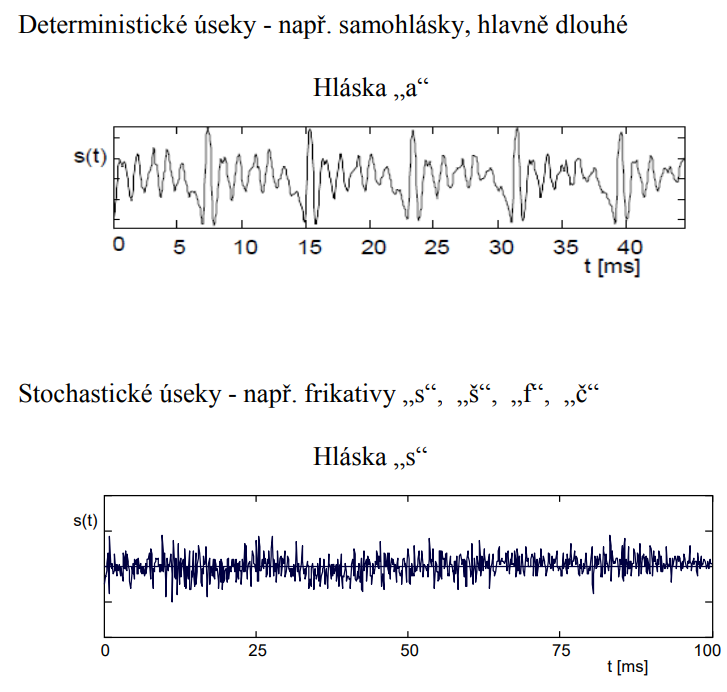
\includegraphics[width=0.82\textwidth]{hlaska_a_hlaska-s.png}
  \caption{Priebeh rečového signálu -- hláska ,,a'' (periodický, znelý úsek) a hláska ,,s'' (šumový, neznelý úsek).}
\end{figure}

% ------------------------------------------------------------
\section{Náhodná veličina a jej popis}
% ------------------------------------------------------------

Náhodný jav je idealizovaný výsledok pokusu (napr. hod kockou, nameraná hodnota
šumu). Keď výsledku pokusu priradíme číslo, hovoríme o \textbf{náhodnej
veličine} --- tá môže byť diskrétna (napr. číslo na kocke) alebo spojitá
(napr. okamžité napätie šumu).

\subsection{Hustota rozdelenia pravdepodobnosti}

Hustota rozdelenia pravdepodobnosti $p(x)$ pre spojitú náhodnú veličinu $\xi$
--- predstav si ju ako krivku, ktorá hovorí, kde sa hodnoty veličiny ,,radi
zdržiavajú''. Vysoká hodnota $p(x)$ na nejakom $x$ znamená, že táto hodnota
nastáva často; nízka znamená, že je zriedkavá. Platia pre ňu tri základné
vlastnosti:
\begin{itemize}
  \item $p(x) \geq 0$ \quad (pravdepodobnosť nemôže byť záporná)
  \item Pravdepodobnosť, že $\xi$ padne do intervalu $\langle a,b\rangle$:
    \[
      P(a \leq \xi \leq b) = \int_a^b p(x)\, dx
    \]
  \item Pravdepodobnosť, že $\xi$ je kdekoľvek, musí byť 1:
    \[
      P(-\infty < \xi < \infty) = \int_{-\infty}^{+\infty} p(x)\, dx = 1
    \]
\end{itemize}

\subsection{Distribučná funkcia}

Distribučná funkcia $F(x) = P(\xi < x)$ je kumulatívna suma hustoty ---
hovorí, aká je pravdepodobnosť, že veličina nadobudne hodnotu menšiu ako $x$.
Je to neklesajúca funkcia, $F(-\infty) = 0$, $F(+\infty) = 1$. Platí:
\[
  p(x) = \frac{dF(x)}{dx}, \qquad F(x) = \int_{-\infty}^{x} p(\alpha)\, d\alpha
\]
Pre diskrétnu veličinu má tvar schodovej funkcie, pre spojitú plynulej krivky.

\begin{figure}[H]
  \centering
  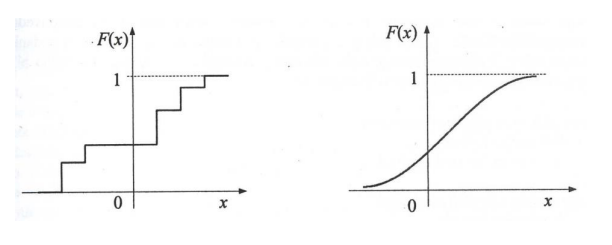
\includegraphics[width=0.82\textwidth]{diskretna_a_spojita_distribucna_funkcia.png}
  \caption{Distribučná funkcia $F(x)$ pre diskrétnu (schodovitá) a spojitú (plynulá) náhodnú veličinu.}
\end{figure}

\subsection{Normálne (Gaussovo) rozdelenie}

Najdôležitejší typ rozdelenia v praxi:
\[
  p(x) = \frac{1}{\sigma\sqrt{2\pi}}
  \exp\!\left[-\frac{(x-\mu)^2}{2\sigma^2}\right]
\]
kde:
\begin{itemize}
  \item $\mu$ --- stredná hodnota [rovnaká jednotka ako $x$]: poloha vrcholu
        krivky (kde sa hodnoty najviac sústreďujú)
  \item $\sigma$ --- smerodajná odchýlka [rovnaká jednotka ako $x$]: šírka
        krivky (čím väčšia $\sigma$, tým ,,rozliata'' krivka, tým väčší
        rozptyl hodnôt)
\end{itemize}
Gaussovo rozdelenie je kľúčové, pretože mnohé reálne šumy ho spĺňajú (napr.
tepelný šum rezistoru). Pre $\mu = 0$ a $\sigma = 1$ ide o normované normálne
rozdelenie.

% ------------------------------------------------------------
\section{Momenty -- číselné charakteristiky náhodnej veličiny}
% ------------------------------------------------------------

Namiesto úplného popisu pomocou $p(x)$ stačí v praxi poznať niekoľko
číselných charakteristík nazývaných \textbf{momenty}. Čím vyšší rád momentu,
tým ,,jemnejšiu'' vlastnosť rozdelenia popisuje.

\subsection{Obecný moment $k$-tého rádu}

Hovorí, aká je priemerná hodnota $x^k$, váhovaná hustotou. Pre spojitú
veličinu:
\[
  m_k = \int_{-\infty}^{+\infty} x^k \, p(x)\, dx
\]
Pre diskrétnu veličinu s možnými hodnotami $x_i$ a pravdepodobnosťami
$P\{x_i\}$:
\[
  m_k = \sum_{i} x_i^k \, P\{x_i\}
\]
kde $x_i$ sú jednotlivé možné hodnoty veličiny a $P\{x_i\}$ je pravdepodobnosť
výskytu hodnoty $x_i$.

\subsection{Centrálny moment $k$-tého rádu}

To isté, ale odčítame strednú hodnotu $\mu$ --- meriame odchýlky od stredu.
Pre spojitú veličinu:
\[
  m_k = \int_{-\infty}^{+\infty} (x - \mu)^k \, p(x)\, dx
\]
Pre diskrétnu veličinu:
\[
  m_k = \sum_{i} (x_i - \mu)^k \, P\{x_i\}
\]

Zmysel: obecný moment $m_1$ nám dá strednú hodnotu, ale ak chceme vedieť, ako
sú hodnoty \emph{rozptýlené okolo stredu}, potrebujeme centrálne momenty (kde
od každej hodnoty $x_i$ najprv odčítame stred $\mu$).

\subsection{Najdôležitejšie momenty}

\begin{itemize}
  \item $m_1$ (obecný, $k=1$) $= \mu$ \textbf{-- stredná hodnota}: priemerná
        hodnota, ťažisko rozdelenia
  \item $m_2$ (centrálny, $k=2$) $= D$ \textbf{-- disperzia (rozptyl)}: priemerná
        kvadratická odchýlka od $\mu$ --- miera toho, ako sú hodnoty
        ,,roztrúsené'' okolo stredu; jednotka je $[x]^2$
  \item $m_3$ (centrálny, $k=3$) -- \textbf{šikmosť}: miera nesymetrie
        rozdelenia okolo stredu
  \item $m_4$ (centrálny, $k=4$) -- \textbf{špičatosť}: miera toho, či je
        rozdelenie zaostrejšie alebo plochejšie ako Gaussovo
\end{itemize}

\textbf{Smerodajná odchýlka}: $\sigma = \sqrt{D}$ --- má rovnaké jednotky
ako signál, priamo interpretovateľná ako ,,typická odchýlka'' od strednej
hodnoty.

% ------------------------------------------------------------
\section{Náhodný proces}
% ------------------------------------------------------------

Náhodný signál popisujeme pojmom \textbf{náhodný proces} $\{\xi_t\}$ --- ide
o sústavu náhodných veličín definovaných v čase. Každé konkrétne meranie
(realizácia) dáva jednu časovú krivku, ale celý proces je reprezentovaný
množinou všetkých možných realizácií. Predstav si to tak: spustíš rovnaký
experiment (napr. meranie šumu rezistoru) 100-krát --- každé meranie dá inú
krivku, ale všetky pochádzajú z toho istého procesu.

\begin{figure}[H]
  \centering
  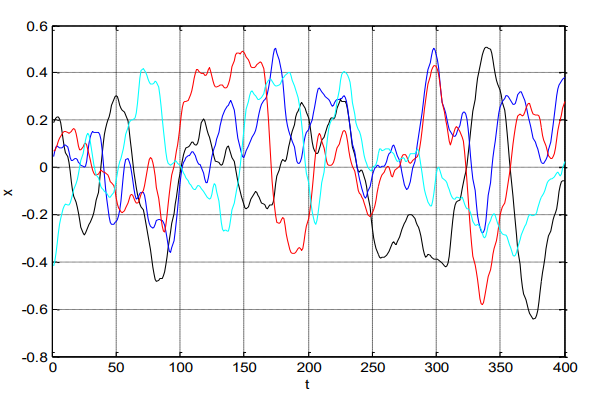
\includegraphics[width=0.82\textwidth]{viacero_realizacii_nahodneho_sumu.png}
  \caption{Množina realizácií náhodného procesu -- šum kovového rezistoru (každá krivka = jedno meranie).}
\end{figure}

\subsection{Stredná hodnota}

Stredná hodnota náhodného procesu v čase $t$ --- priemer cez všetky možné
hodnoty v danom okamihu, váhovaný hustotou $p(x,t)$:
\[
  a(t) = \int_{-\infty}^{+\infty} x \, p(x,t)\, dx
\]
kde $x$ je integrovaná premenná (možné hodnoty signálu) a $p(x,t)$ je hustota
rozdelenia v čase $t$. V praxi sa odhaduje ako aritmetický priemer $K$
realizácií v okamihu $t$:
\[
  \hat{a}(t) = \frac{1}{K}\sum_{k=1}^K x_k(t)
\]
kde $K$ je počet realizácií a $x_k(t)$ je hodnota $k$-tej realizácie v čase
$t$.

\subsection{Disperzia (rozptyl)}

Disperzia v čase $t$ --- priemerná kvadratická odchýlka hodnôt od strednej
hodnoty $a(t)$ v danom okamihu:
\[
  D(t) = \int_{-\infty}^{+\infty} \bigl[x - a(t)\bigr]^2 \, p(x,t)\, dx
\]
kde $x$ je integrovaná premenná (možné hodnoty signálu) a $a(t)$ je stredná
hodnota procesu v čase $t$. Čím väčšia $D(t)$, tým viac sú realizácie
v čase $t$ ,,roztrúsené'' okolo strednej hodnoty --- tým väčší výkon šumu.

\textbf{Smerodajná odchýlka} procesu: $\sigma(t) = \sqrt{D(t)}$

% ------------------------------------------------------------
\section{Autokorelačná funkcia (AKF)}
% ------------------------------------------------------------

AKF popisuje vzájomnú závislosť hodnôt signálu v dvoch rôznych časových
okamihoch --- hovorí, nakoľko ,,pamätá'' signál svoju minulosť. Pre
stacionárny náhodný proces závisí len od časového rozdielu $\tau = t_2 - t_1$,
nie od absolútneho času:
\[
  R(\tau) = E\{\xi(t) \cdot \xi(t+\tau)\}
\]
kde:
\begin{itemize}
  \item $\tau$ --- časové posunutie (oneskorenie) medzi dvoma okamihmi
        porovnávania [s]
  \item $\xi(t)$ --- hodnota náhodného procesu v čase $t$
  \item $\xi(t+\tau)$ --- hodnota toho istého procesu o $\tau$ neskôr
  \item $E\{\cdot\}$ --- operátor stredovania (priemer cez realizácie)
\end{itemize}

\textbf{Intuitívne:} pre $\tau = 0$ porovnávame signál sám so sebou ---
výsledok je maximálny. Pre rastúce $\tau$ sa hodnoty čoraz viac ,,rozídu''
a korelácia klesá. Pre biely šum klesne okamžite na nulu (žiadna pamäť), pre
hladký signál klesá pomaly.

\subsection{Vlastnosti AKF stacionárneho procesu}

\begin{itemize}
  \item \textbf{Maximum v $\tau = 0$}:
    \[
      R(0) = E\{\xi^2(t)\} = D + a^2
    \]
    čo je stredný výkon signálu. Pre nulový jednosmerný priebeh ($a = 0$):
    $R(0) = D = \sigma^2$
  \item \textbf{Párna funkcia}: $R(\tau) = R(-\tau)$ --- pohľad dopredu
        a dozadu v čase dáva rovnaký výsledok
  \item Pre veľké $\tau$ klesá k $a^2$ --- signál ,,zabudne'' svoju minulosť,
        ostane len prínos strednej hodnoty
  \item Disperzia $D$ v grafe AKF je výška poklesu od maxima $R(0)$
        k asymptote $a^2$, teda $D = R(0) - a^2$
  \item U procesov s nulovou strednou hodnotou ($a = 0$) má smerodajná
        odchýlka $\sigma$ význam efektívnej hodnoty signálu a platí
        $P = X_{ef}^2 = D = \sigma^2$ (výkon na záťaži 1\,$\Omega$)
\end{itemize}

\begin{figure}[H]
  \centering
  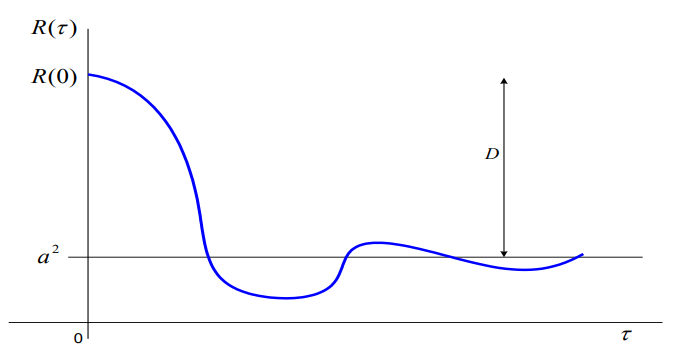
\includegraphics[width=0.82\textwidth]{tvar_autokorelacnej_funkcie.png}
  \caption{AKF stacionárneho náhodného signálu s vyznačenými hodnotami $R(0)$, $a^2$ a $D$.}
\end{figure}

% ------------------------------------------------------------
\section{Stacionarita}
% ------------------------------------------------------------

Náhodný proces je \textbf{stacionárny}, ak jeho štatistické charakteristiky
nezávisia od posunutia počiatku časovej osi --- sú rovnaké kdekoľvek v čase.
Formálne platí:
\[
  F(x,t) \to F(x), \qquad a(t) \to a, \qquad D(t) \to D
\]
\[
  p(x_1,x_2,t_1,t_2) \to p(x_1,x_2,\tau), \qquad \tau = t_2 - t_1
\]

\textbf{Predstav si to takto:} ak by si vystrihol ľubovoľný úsek záznamu
a vypočítal štatistiku, vždy dostaneš rovnaké výsledky. Typický príklad
stacionárneho procesu: tepelný šum rezistoru. Nestacionárny: zvuk záchranky,
ktorá mení frekvenciu --- jej štatistika sa mení s časom.

\begin{figure}[H]
  \centering
  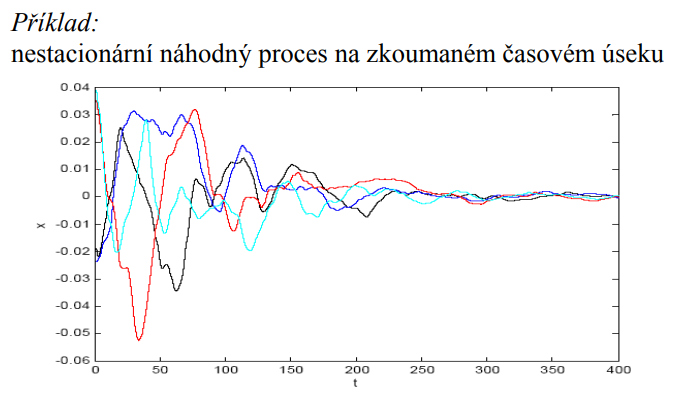
\includegraphics[width=0.82\textwidth]{priklad_nestacionarneho_nahodneho_procesu.png}
  \caption{Nestacionárny náhodný proces -- amplitúda realizácií sa mení s časom.}
\end{figure}

% ------------------------------------------------------------
\section{Ergodicita}
% ------------------------------------------------------------

Ergodický proces je stacionárny proces s ešte silnejšou vlastnosťou:
\textbf{všetky realizácie majú rovnaké štatistické vlastnosti} a stačí preto
skúmať jedinú (ľubovoľnú) realizáciu. Praktický dôsledok: časový priemer
vypočítaný z jednej dlhej realizácie = priemer cez realizácie v danom
okamihu.

Bez predpokladu ergodicity by sme pre odhad strednej hodnoty potrebovali
súbežne veľa meraní --- čo je v praxi často nemožné. Podmienkou je dostatočne
dlhý čas záznamu.

\textbf{Príklad:} šum rezistoru je ergodický --- jedno dlhé meranie stačí na
spoľahlivé určenie všetkých štatistík.

\begin{figure}[H]
  \centering
  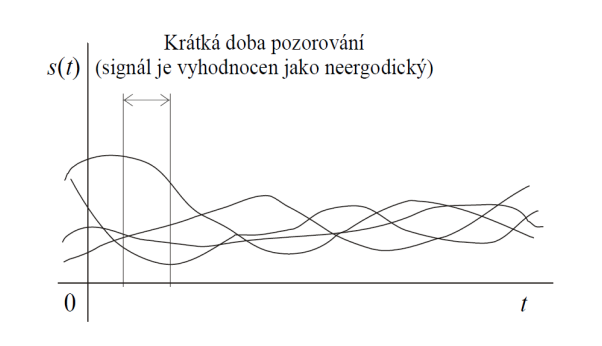
\includegraphics[width=0.82\textwidth]{priklad_ergodicity.png}
  \caption{Ergodicita -- pri krátkej dobe pozorovania sa realizácie zdajú rôzne; pri dostatočne dlhej sú štatisticky zhodné.}
\end{figure}

% ------------------------------------------------------------
\section{Spektrálna hustota výkonu $G(\omega)$}
% ------------------------------------------------------------

Kým AKF opisuje náhodný signál v čase, spektrálna hustota výkonu $G(\omega)$
opisuje, \textbf{ako je rozložený výkon signálu po frekvenciách} --- koľko
výkonu sa nachádza v každom frekvenčnom pásme. Funkcia je párna
($G(\omega) = G(-\omega)$) a nezáporná.

\textbf{Celkový stredný výkon} stacionárneho ergodického procesu:
\[
  P = \int_{-\infty}^{+\infty} G(\omega)\, d\omega
\]
kde $\omega$ je uhlová frekvencia [rad/s].

\textbf{Výkon v pásme} od $\omega_1$ do $\omega_2$:
\[
  P = 2\int_{\omega_1}^{\omega_2} G(\omega)\, d\omega
\]
(faktor 2 kvôli symetrii -- pre záporné frekvencie platí to isté).

\textbf{Biely šum} má konštantnú spektrálnu hustotu $G(\omega) = G$ pre
všetky frekvencie --- analogia k bielému svetlu, ktoré obsahuje všetky farby
rovnomerne. V reálnom svete neexistuje (mal by nekonečný výkon), ale je
dôležitý ako matematický model šumu.

\textbf{Meranie $G(\omega)$ v praxi} pásmovým filtrom so šírkou pásma $b$
a stredným kmitočtom $\omega_c$. Nameraný výkon $P(b, \omega_c)$ na výstupe
filtra dá:
\[
  G(\omega_c) \approx \frac{P(b,\, \omega_c)}{2b}
\]
kde $b$ je šírka pásma filtra [rad/s] a $P(b, \omega_c)$ je stredný výkon
nameraný na výstupe filtra. Čím užší filter, tým presnejší odhad spektra
v danom bode.

\begin{figure}[H]
  \centering
  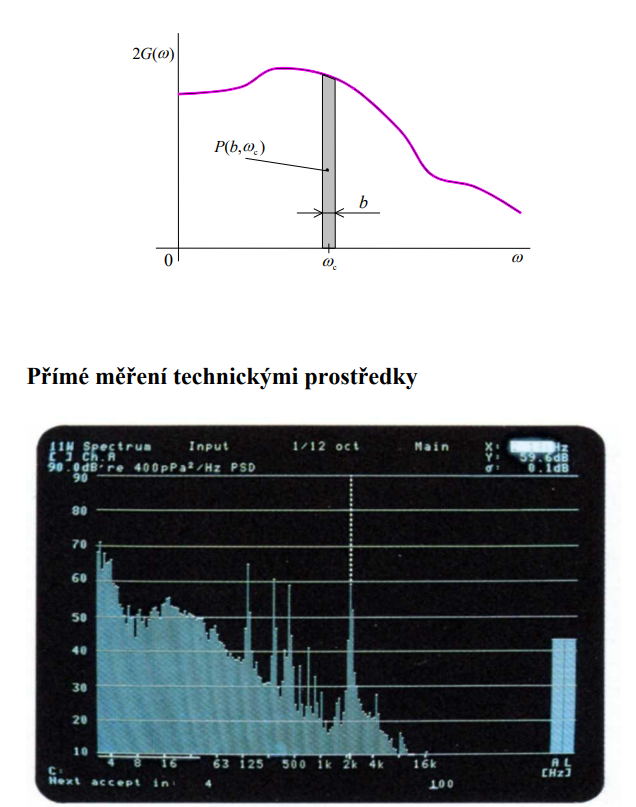
\includegraphics[width=0.82\textwidth]{graf_merania_priemyselného_hluku_a_schema_principu_merania.png}
  \caption{Schéma merania $G(\omega)$ pásmovým filtrom (hore) a reálne namerané spektrum priemyselného hluku (dole).}
\end{figure}

% ------------------------------------------------------------
\section{Typy šumov}
% ------------------------------------------------------------

Náhodné signály sa delia podľa rôznych kritérií:
\begin{itemize}
  \item \textbf{Stacionárny šum} --- spektrálne vlastnosti konštantné v čase
        (napr. hluk ventilátora, tepelný šum); oproti tomu \textbf{nestacionárny}
        --- meniace sa vlastnosti (siréna záchranky, štekat psa).
  \item \textbf{Bielý šum} --- rovnomerné spektrum;
        \textbf{farebný šum} --- získaný pásmovým filtrovaním bieleho
        (ružový, červený\ldots).
  \item \textbf{Aditivný šum} --- pripočítava sa k užitočnému signálu, nie je
        s ním korelovaný (napr. hluk pozadia pri nahrávaní mikrofónom).
  \item \textbf{Konvolučný šum} --- vzniká skreslením signálu v prenosovom
        kanáli, má väzbu na užitočný signál (napr. odrazy, dozvuk v miestnosti).
\end{itemize}

% ============================================================
% OKRUH 2
% 
\chapter{Lineárna filtrácia signálov -- filtre FIR a IIR}

% ------------------------------------------------------------
\section{Čo je filter a čo robí}
% ------------------------------------------------------------

Filter je systém, ktorý \textbf{selektívne prepúšťa určité frekvencie
a potláča iné}. Ideálny filter má pravoúhlu frekvenčnú charakteristiku
(dokonalé prepustenie v pásme, dokonalé potlačenie mimo neho); reálne filtre
majú pozvoľnejší prechod a istú mieru zvlnenia. Podľa prepúšťaného pásma
rozlišujeme:
\begin{itemize}
  \item \textbf{Dolná priepusť (DP)} --- prepúšťa nízke frekvencie
  \item \textbf{Horná priepusť (HP)} --- prepúšťa vysoké frekvencie
  \item \textbf{Pásmová priepusť (PP)} --- prepúšťa pásmo uprostred
  \item \textbf{Pásmová zádrž (PZ)} --- blokuje pásmo uprostred
\end{itemize}

% ------------------------------------------------------------
\section{Analógové filtre}
% ------------------------------------------------------------

Realizujú sa pasívnymi súčiastkami (R, C, L) alebo aktívne s operačným
zosilňovačom. Návrh prebieha v dvoch etapách.

\subsection{1. etapa -- signálová}

Výber prenosovej funkcie $H(p)$ vhodnou aproximáciou. Pre dolnú priepusť:
\[
  H(p) = \frac{K_0}{1 + k_1 P + k_2 P^2 + \ldots + k_N P^N}
\]
kde:
\begin{itemize}
  \item $K_0$ --- zosilnenie filtra na nulovom kmitočte [bezrozmerné]
  \item $N$ --- rád filtra; čím vyšší, tým strmší prechod medzi priepustným
        a zádrž\-ným pásmom
  \item $k_i$ ($i = 1 \ldots N$) --- koeficienty určujúce typ aproximácie,
        preberajú sa z tabuliek
  \item $P = j\omega/\omega_m$ --- normovaný komplexný kmitočet;
        $\omega_m$ je medzný (návrhový) kmitočet [rad/s]
\end{itemize}

Pre hornú priepusť sa prenosová funkcia získa zámenou $P \to 1/P$ (v obvode
to zodpovedá vzájomnej záméne kondenzátorov a rezistorov). Typ aproximácie
určuje správanie v priepustnom pásme:
\begin{itemize}
  \item \textbf{Butterworthova} --- maximálne plochá charakteristika,
        bez zvlnenia
  \item \textbf{Besselova} --- najlepšia linearita fázy (minimálne fázové
        skreslenie)
  \item \textbf{Čebyševova} --- strmší prechod za cenu zvlnenia v priepustnom
        pásme
\end{itemize}

\begin{figure}[H]
  \centering
  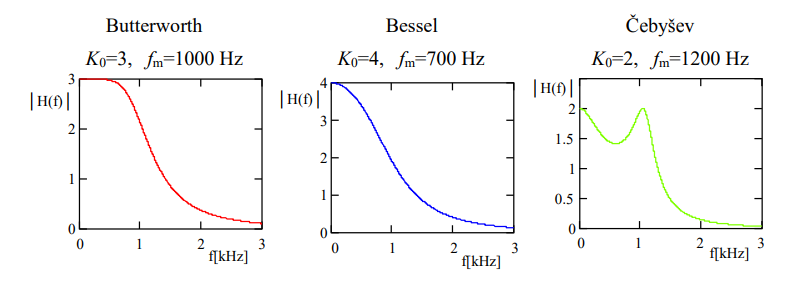
\includegraphics[width=0.82\textwidth]{porovnanie_modulovych_frek_char.png}
  \caption{Porovnanie modulových charakteristík dolnej priepuste -- Butterworth, Bessel, Čebyšev.}
\end{figure}

\subsection{2. etapa -- obvodová}

Na základe zvoleného zapojenia (napr. Sallenov-Keyov obvod) sa z koeficientov
$k_i$ vypočítajú konkrétne hodnoty súčiastok R a C.

% ------------------------------------------------------------
\section{Číslicové filtre -- FIR a IIR}
% ------------------------------------------------------------

Číslicové filtre pracujú s diskrétnymi vzorkami signálu. Výstup $y(n)$ je
určený konvolúciou vstupného signálu $x(n)$ s impulznou odozvou $h(k)$.
Podľa dĺžky impulznej odozvy rozlišujeme dve hlavné triedy.

\subsection{FIR -- Finite Impulse Response (konečná impulzná odozva)}

Výstup závisí len od $N$ posledných vstupných vzorkov:
\[
  y(n) = \sum_{k=0}^{N-1} h(k) \cdot x(n-k)
\]
kde:
\begin{itemize}
  \item $y(n)$ --- aktuálny výstupný vzorek
  \item $x(n-k)$ --- vstupné vzorky: $x(n)$ je aktuálny, $x(n-1)$ je
        o jeden krok starší, atď.
  \item $h(k)$ --- koeficienty filtra (= hodnoty impulznej odozvy
        v diskrétnom čase $k$)
  \item $N$ --- počet koeficientov (rád filtra $+ 1$)
\end{itemize}

Prenosová funkcia v $z$-oblasti:
\[
  H(z) = \sum_{k=0}^{N-1} h(k)\, z^{-k}
\]
kde $z^{-k}$ zodpovedá oneskoreniu o $k$ vzorkov. FIR nemá spätnú väzbu
--- každý výstupný vzorek závisí výlučne od vstupov.

\subsection{IIR -- Infinite Impulse Response (nekonečná impulzná odozva)}

Realizovaný rekurzívnou rovnicou (spätná väzba):
\[
  y(n) = \sum_{k=0}^{N} b_k \cdot x(n-k) \;-\; \sum_{k=1}^{M} a_k \cdot y(n-k)
\]
kde:
\begin{itemize}
  \item $b_k$ --- koeficienty priamej vetvy (váhy vstupných vzorkov $x$;
        $k = 0 \ldots N$)
  \item $a_k$ --- koeficienty spätnoväzbovej vetvy (váhy predchádzajúcich
        výstupov $y$; $k = 1 \ldots M$)
  \item $y(n-k)$ --- výstupné vzorky z minulosti, ktoré sa ,,vracajú'' späť
        do výpočtu
\end{itemize}

Prenosová funkcia:
\[
  H(z) = \frac{\displaystyle\sum_{k=0}^{N} b_k\, z^{-k}}
              {1 + \displaystyle\sum_{k=1}^{M} a_k\, z^{-k}}
\]

\textbf{Intuitívne:} vďaka spätnej väzbe ,,pamätá'' IIR filter svoju vlastnú
minulosť --- impulz na vstupe sa v systéme ,,odráža'' donekonečna (teoreticky),
preto nekonečná odozva. Toto mu dáva veľkú efektivitu: rovnako ostrú
frekvenčnú charakteristiku dosiahne s omnoho menej koeficientmi ako FIR.



% ------------------------------------------------------------
\section{Vlastnosti a porovnanie FIR vs IIR}
% ------------------------------------------------------------

\subsection*{FIR}
\begin{itemize}
  \item Vždy stabilný --- stabilita je garantovaná štruktúrou (žiadna spätná
        väzba nemôže spôsobiť rozkmitanie)
  \item Lineárna fázová charakteristika --- všetky frekvencie sú oneskorené
        o rovnakú dobu, takže tvar signálu nie je skreslený; kľúčové pre reč,
        EKG, dáta
  \item Pre ostrý prechod potrebuje vysoký rád (veľa koeficientov $N$)
        $\to$ dlhší výpočet, väčšia pamäť
  \item Rušivý impulz na vstupe ovplyvní výstup len po dobu $N$ vzorkov,
        potom zmizne
  \item Nemá analógový ekvivalent
\end{itemize}

\subsection*{IIR}
\begin{itemize}
  \item Môže byť nestabilný pri zle navrhnutých koeficientoch (spätná väzba
        môže spôsobiť nárast výstupu do nekonečna)
  \item Nelineárna fázová charakteristika --- rôzne frekvencie sú oneskorené
        rôzne dlho (fázové skreslenie)
  \item Nízky rád (typicky do 10) --- výpočtovo efektívny
  \item Krátky rušivý impulz môže prostredníctvom spätnej väzby trvale
        ovplyvniť výstup
  \item Analógové filtre sa dajú priamo previesť na IIR
        (metóda bilineárnej transformácie)
\end{itemize}

\noindent\textbf{Odporúčanie pre prax:}
\begin{itemize}
  \item \textbf{IIR} --- ak je hlavnou požiadavkou ostrá frekvenčná selekcia
        s čo najmenším počtom koeficientov
  \item \textbf{FIR} --- ak je dôležitá lineárna fáza, alebo počet
        koeficientov nie je problémom
\end{itemize}

% ------------------------------------------------------------
\section{Metódy návrhu číslicových filtrov v MATLABe}
% ------------------------------------------------------------

Všetky kmitočty použité v návrhu sú normované v rozsahu 0 až 1, kde 1
zodpovedá polovici vzorkovacieho kmitočtu $f_{vz}/2$. Napríklad pre medzný
kmitočet $f_m = 300$\,Hz a vzorkovací kmitočet 1000\,Hz (teda $f_{vz}/2 =
500$\,Hz) sa zadáva $W_p = 300/500 = 0{,}6$.

\textbf{Pre IIR} návrh prebieha v dvoch krokoch:

\noindent\textit{1. Výpočet rádu filtra $n$ a návrhového medzného kmitočtu $W_n$:}

\begin{center}
\begin{tabular}{ll}
  \toprule
  \textbf{Typ filtra} & \textbf{Funkcia} \\
  \midrule
  Butterworth        & \texttt{[n, Wn] = buttord(Wp, Ws, Rp, As)} \\
  Chebyshev I        & \texttt{[n, Wn] = cheb1ord(Wp, Ws, Rp, As)} \\
  Chebyshev II       & \texttt{[n, Wn] = cheb2ord(Wp, Ws, Rp, As)} \\
  Eliptický (Cauer)  & \texttt{[n, Wn] = ellipord(Wp, Ws, Rp, As)} \\
  \bottomrule
\end{tabular}
\end{center}

\noindent kde $W_p$ je normovaný medzný kmitočet v priepustnom pásme,
$W_s$ v zádrži (oba 0--1), $R_p$ je maximálne zvlnenie v priepustnom pásme
[dB], $A_s$ je minimálny útlm v zádrži [dB].

\noindent\textit{2. Výpočet koeficientov $b$ (čitateľ) a $a$ (menovateľ):}

\begin{center}
\begin{tabular}{ll}
  \toprule
  \textbf{Typ filtra} & \textbf{Funkcia} \\
  \midrule
  Butterworth        & \texttt{[b, a] = butter(n, Wn, options)} \\
  Chebyshev I        & \texttt{[b, a] = cheby1(n, Rp, Wn, options)} \\
  Chebyshev II       & \texttt{[b, a] = cheby2(n, As, Wn, options)} \\
  Eliptický          & \texttt{[b, a] = ellip(n, Rp, As, Wn, options)} \\
  \bottomrule
\end{tabular}
\end{center}

\noindent Filtrácia signálu $x$: \quad \texttt{y = filter(b, a, x)}

\textbf{Pre FIR}: najčastejšie metóda okien --- navrhnutá impulzná odozva
sa váhuje okienkovou funkciou (Hanning, Hamming, Kaiser) na potlačenie
vedľajších lalokov v zádrži. V MATLABe napr. \texttt{fir1}, \texttt{firpm}.



% ------------------------------------------------------------
\section{Spôsoby realizácie}
% ------------------------------------------------------------

Číslicové filtre sa realizujú:
\begin{itemize}
  \item \textbf{Softvérovo} --- výpočet rovnice $y(n)$ vzorku po vzorku
        v procesore alebo DSP čipe
  \item \textbf{Hardvérovo} --- obvody FPGA alebo ASIC implementujúce sieť
        násobiček a sčítavačov: pre FIR priama (transversálna) štruktúra,
        pre IIR rekurzívna štruktúra so spätnou väzbou
\end{itemize}

Vizualizácia vlastností filtra v MATLABe:
\begin{itemize}
  \item \texttt{freqz(b, a, K, fvz)} --- modulová a fázová frekvenčná
        charakteristika ($K$ bodov, vzorkovací kmitočet \texttt{fvz})
  \item \texttt{impz(b, a, N)} --- impulzná odozva ($N$ vzorkov)
  \item \texttt{zplane(b, a)} --- mapa núl a pólov v $z$-rovine
\end{itemize}

\begin{figure}[H]
  \centering
  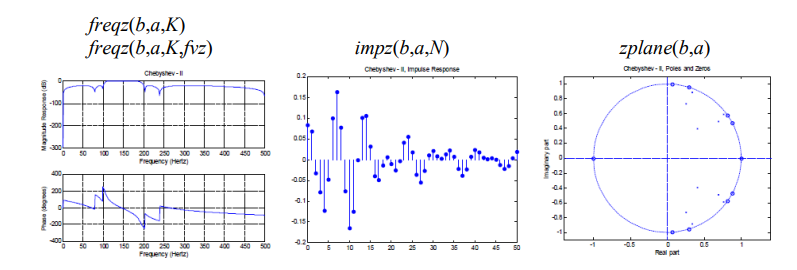
\includegraphics[width=0.82\textwidth]{frekvencna_char_impulzna_char_mapa_polov.png}
  \caption{Frekvenčná charakteristika, impulzná odozva a mapa pólov/núl číslicového filtra Chebyshev~II v MATLABe.}
\end{figure}

% ============================================================
% OKRUH 3
% ============================================================
\chapter{Lineárna predikcia signálu (LPC)}

% ------------------------------------------------------------
\section{Definícia lineárnej predikcie}
% ------------------------------------------------------------

Lineárna predikcia (LPC --- Linear Predictive Coding) spočíva v myšlienke,
že \textbf{aktuálny vzorek signálu vieme odhadnúť ako váhovanú sumu
predchádzajúcich vzorkov} toho istého signálu. Predikovaná hodnota $n$-tého
vzorka:
\[
  \hat{s}(n) = \sum_{m=1}^{M} a_m \cdot s(n-m)
\]
kde:
\begin{itemize}
  \item $\hat{s}(n)$ --- predikovaná (odhadnutá) hodnota vzorka s indexom $n$
  \item $s(n-m)$ --- skutočné hodnoty predchádzajúcich vzorkov: $s(n-1)$ je
        bezprostredne predchádzajúci, $s(n-2)$ je o dva kroky starší, atď.
  \item $a_m$ --- predikčné (LPC) koeficienty ($m = 1 \ldots M$); hovorí sa
        im aj ,,váhy''
  \item $M$ --- rád prediktora: koľko predchádzajúcich vzorkov použijeme
\end{itemize}

\textbf{Intuitívne:} je to podobné, ako keby si pri predpovedaní počasia
dnes ráno vychádzal z teplôt posledných $M$ dní --- každý deň má svoju váhu
$a_m$.

\textbf{Chyba predikcie} (reziduál) $e(n)$ --- rozdiel medzi skutočnou
a predikovanou hodnotou:
\[
  e(n) = s(n) - \hat{s}(n) = s(n) - \sum_{m=1}^{M} a_m \cdot s(n-m)
\]
kde $e(n)$ je chyba predikcie $n$-tého vzorka [rovnaká jednotka ako $s(n)$].

% ------------------------------------------------------------
\section{Výpočet koeficientov -- minimalizácia chyby}
% ------------------------------------------------------------

Cieľom LPC analýzy je nájsť koeficienty $a_m$ tak, aby bola celková
kvadratická chyba cez segment $N$ vzorkov minimálna:
\[
  Er = \sum_{n=1}^{N} e^2(n)
     = \sum_{n=1}^{N} \left[s(n) - \sum_{m=1}^{M} a_m \cdot s(n-m)\right]^2
\]
kde $Er$ je celková kvadratická chyba predikcie, $N$ je dĺžka spracovávaného
segmentu a $n$ je index vzorka v segmente.

Minimalizácia $Er$ parciálnymi deriváciami podľa každého $a_m$ vedie na
sústavu $M$ lineárnych rovníc --- \textbf{Yule-Walkerove rovnice}
v maticovom tvare:
\[
\begin{pmatrix}
  R(0)   & R(1)   & R(2)   & \cdots & R(M-1) \\
  R(1)   & R(0)   & R(1)   & \cdots & R(M-2) \\
  \vdots &        &        & \ddots & \vdots \\
  R(M-1) & R(M-2) & R(M-3) & \cdots & R(0)
\end{pmatrix}
\begin{pmatrix} a_1 \\ a_2 \\ \vdots \\ a_M \end{pmatrix}
=
\begin{pmatrix} R(1) \\ R(2) \\ \vdots \\ R(M) \end{pmatrix}
\]
kde $R(k)$ je autokorelačná funkcia segmentu signálu pri oneskorení $k$
--- teda miera podobnosti signálu so sebou samým posunutým o $k$ vzorkov.
Matica je Toeplitzová (symetrická, každá diagonála má rovnaké hodnoty), čo
umožňuje efektívne riešenie Levinsonovým-Durbinovým algoritmom.

\textbf{Prakticky:} čím je signál periodickejší (napr. znelá samohláska),
tým väčšia $R(k)$ pre $k = $ perióda, tým lepšie koeficienty dokážu
predpovedať nasledujúce vzorky. Šumové (neznelé) úseky (napr.\ hláska ,,s'')
majú $R(k) \approx 0$ pre $k > 0$ --- predikcia funguje oveľa horšie.

\begin{figure}[H]
  \centering
  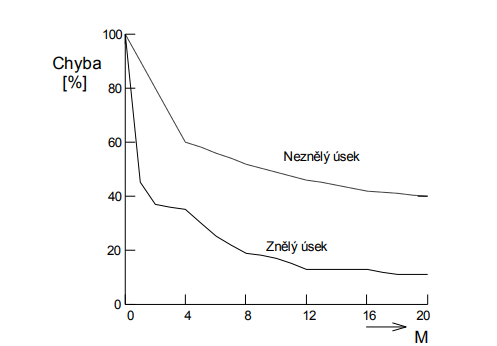
\includegraphics[width=0.82\textwidth]{zavislost_chyby_zneleho_a_nezneleho_useku.png}
  \caption{Závislosť chyby predikcie na počte koeficientov $M$ pre znelý a neznelý úsek reči.}
\end{figure}

% ------------------------------------------------------------
\section{Využitie pre reštauráciu signálu}
% ------------------------------------------------------------

Ak poznáme koeficienty $a_m$ a máme k dispozícii predchádzajúce vzorky,
vieme dopočítať chýbajúci alebo poškodený vzorek:
\[
  \hat{s}(n) = \sum_{m=1}^{M} a_m \cdot s(n-m)
\]
Namiesto predikcie budúcich vzorkov rekonštruujeme chýbajúce. Funguje tým
lepšie, čím je signál viac ,,predvídateľný'' --- teda pre hladké, kváziperiodické
úseky (samohlásky, hudba). Pre šumové úseky je reštaurácia menej presná.

% ------------------------------------------------------------
\section{Využitie pre spektrálnu analýzu -- LPC spektrum}
% ------------------------------------------------------------

Z predikčných koeficientov $a_m$ možno pomocou $z$-transformácie vypočítať
\textbf{LPC spektrum}:
\[
  LS(f) = \left|\frac{1}{1 - \displaystyle\sum_{m=1}^{M} a_m \cdot
  z^{-m}}\right|^2_{\!\!z\,=\,\exp(j2\pi f/f_{vz})}
\]
kde:
\begin{itemize}
  \item $f$ --- frekvencia spektra (nezávislá premenná) [Hz],
        v rozsahu $0$ až $f_{vz}/2$
  \item $f_{vz}$ --- vzorkovací kmitočet signálu [Hz]
  \item $a_m$ --- predikčné koeficienty ($m = 1 \ldots M$)
  \item $z^{-m}$ --- oneskorenie o $m$ vzorkov v $z$-oblasti; dosadením
        $z = e^{j2\pi f/f_{vz}}$ prechádzame do frekvenčnej oblasti
\end{itemize}

LPC spektrum má tvar \textbf{vyhladenej obálky FFT spektra} --- potláča
detailné kolísanie a zvýrazňuje spektrálne vrcholy. Miera vyhlazenia závisí
od $M$: nízke $M$ $\to$ hrubá aproximácia (len celkový sklon), vyššie $M$
$\to$ jemnejší tvar s viditeľnými vrcholmi. Pre reč typicky $M = 10$--$16$
koeficientov.

\begin{figure}[H]
  \centering
  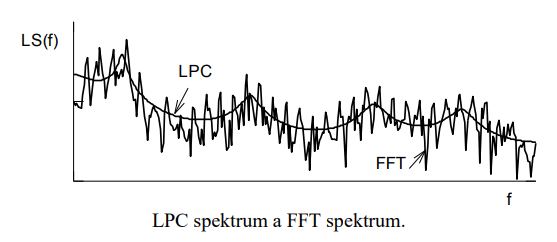
\includegraphics[width=0.82\textwidth]{porovnanie_LPC_a_FFT_spektra.png}
  \caption{LPC spektrum (vyhladená obálka) vs.\ FFT spektrum pre ten istý segment reči.}
\end{figure}

\begin{figure}[H]
  \centering
  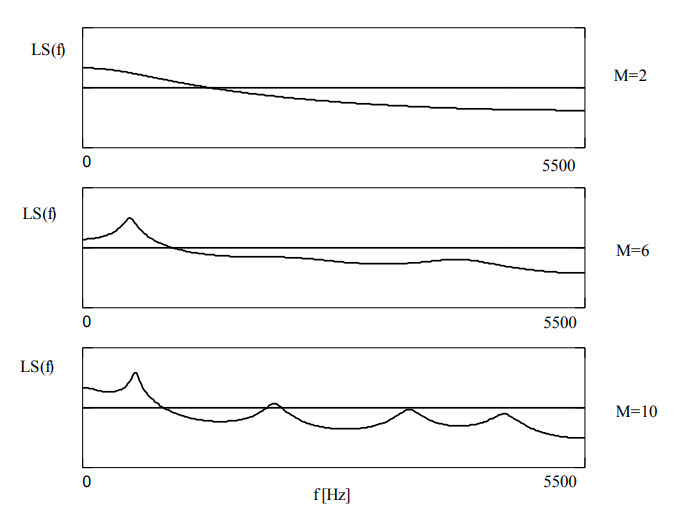
\includegraphics[width=0.82\textwidth]{vplyv_poctu_koeficientov_na_LPC.png}
  \caption{Vplyv počtu koeficientov $M$ na tvar LPC spektra ($M = 2, 6, 10$).}
\end{figure}

Lokálne maximá LPC spektra zodpovedajú \textbf{formantovým kmitočtom} ---
rezonančným frekvenciám vokálneho traktu pri tvorbe danej hlásky. Tieto
možno určiť priamo z pólov $z$-transformácie (korene rovnice
$1 - \sum_{m=1}^{M} a_m \cdot z^{-m} = 0$), čo nevyžaduje ani vykresľovanie
spektra.

% ------------------------------------------------------------
\section{Význam pre rozpoznávanie reči}
% ------------------------------------------------------------

LPC je kľúčová metóda v spracovaní reči z viacerých dôvodov:

\textbf{1. Model hlasového traktu.} Reč vzniká excitáciou (hlasivky
generujú periodický sled impulzov pre znelé hlásky, alebo šum pre neznelé)
filtrovanou vokálnym traktom. LPC model tento filter priamo parametrizuje
--- koeficienty $a_m$ charakterizujú tvar vokálneho traktu pre danú hlásku
v danom časovom okamihu. Tá istá hláska ,,a'' bude mať u rôznych ľudí rôzne
spektrum, ale LPC koeficienty zachytia tvar spektra nezávisle od výšky
hlasu.

\textbf{2. Kompaktná reprezentácia.} Namiesto tisícok vzoriek v 20\,ms
segmente stačí 10--16 predikčných koeficientov. To dramaticky redukuje objem
dát --- podstatné pre kódovanie a prenos reči.

\textbf{3. Príznakové vektory pre klasifikátor.} LPC koeficienty (alebo
z nich odvodené cepstrálne koeficienty LPCC) tvoria príznakové vektory pre
klasifikátory (HMM, DTW, neurónové siete). Každý segment reči je opísaný
vektorom $(a_1, a_2, \ldots, a_M)$ a rozpoznávač hľadá, ku ktorej triede
(hláske, slovu) je tento vektor najbližšie.

\textbf{4. Rozlíšenie znelosti.} Znelé úseky sa predikujú s malou chybou
$e(n)$, neznelé s veľkou. Energia reziduálu je preto sama o sebe príznakom
znelosti --- priamo využiteľné pri segmentácii reči.


\subsection*{Zhrnutie -- význam a využitie metódy LPC}

\begin{itemize}
  \item \textbf{Predpovídání budoucích vzorků} --- na základe koeficientov $a_m$
        a predchádzajúcich vzorkov možno odhadnúť nasledujúce vzorky signálu
        v časovom priebehu (využitie pri kompresii, reštaurácii, kódovaní reči)
  \item \textbf{Výpočet spektra (modulového)} --- z koeficientov $a_m$ sa
        priamo vypočíta vyhladené LPC spektrum $LS(f)$, ktoré reprezentuje
        spektrálnu obálku signálu a polohu formantov
  \item \textbf{Využití LPC koeficientů ke klasifikaci signálů} --- koeficienty
        $a_m$ (alebo z nich odvodené cepstrálne koeficienty LPCC) tvoria
        príznakové vektory pre klasifikátory rozpoznávania reči (HMM, DTW,
        neurónové siete)
\end{itemize}

% ============================================================
%\end{document}